\section{Project Pada Gitlab}

Pada bab sebelumnya kita telah mempraktekan pengoprasian apa saja yang dapat dilakukan pada github, seperti dengan membuat repository, membaca pull request, melakukan merge request dan sebagainya. Pada section kali ini kita kan mempelajari bagaimana pengoprasian pada gitlab. Pertama yang akan dijelaskan disini adalah bagaimana membuat project atau repository pada gitlab. 

Skenarionya sama dengan github dimana kita akan melakukan kontribusi terhadap sebuah project/repo \textit{Open Source} pada Gitlab. Pada dasarnya kita akan mempelajari bagaimana caranya untuk ikut berkontribusi kepada project \textit{Open Source} yang ada pada Gitlab. Untuk membantu para user yang baru memiliki akun gitlab, pertama-tama akan dijelaskan terlebih dahulu bagaimana melakukan setting konfigurasi key agar kita dapat mengakses semua project/repo dari profil kita. Berikut adalah langkah-langkah yang diperlukan untuk melakukan setting konfigurasi key :
\begin{enumerate}
\item Buat akun terlebih dahulu pada alamat \textbf{www.gitlab.com}
\item Install \textbf{Git Bash} dari alamat \textit{git-scm/downloads} pada komputer anda, kemudian buka aplikasi git bash setelah melakukan penginstallan.
\item Pastikan kita telah berada di \textit{home directory} dengan mengetikan perintah \textbf{cd} kemudian klik enter. Setelah itu untuk mengetahui posisi dimana direktori kita berada, ketikkan perintah \textbf{pwd} kemudian enter.
\item Lakukan proses generate key dengan perintah \textbf{ssh-keygen} seperti pada gambar \ref{k1}
\subitem 
\begin{figure}[!htbp]
\centerline{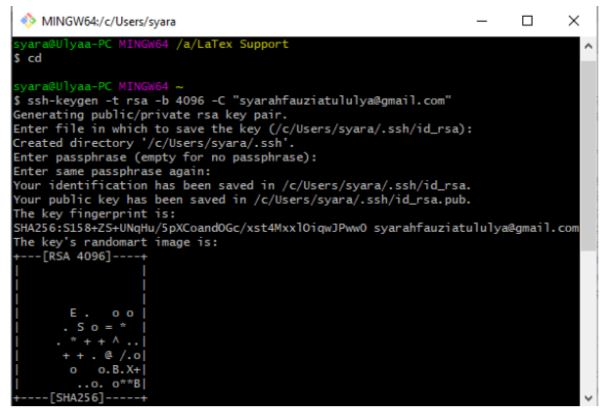
\includegraphics[width=.75\textwidth]{Figures/gitlab/SSH.JPG}}
\caption{Proses Generate Key Gitlab}
\label{fig:k1}
\end{figure}
\item Hasil outputnya seperti pada gambar \ref{s1}
\subitem
\begin{figure}[!htbp]
\centerline{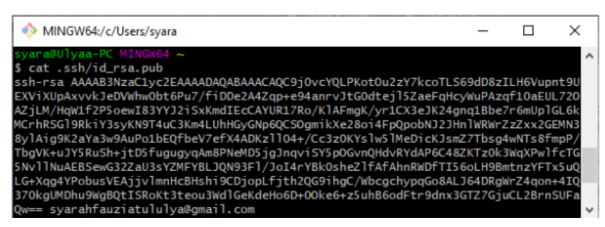
\includegraphics[width=.75\textwidth]{Figures/gitlab/SSH2.JPG}}
\caption{Hasil Output SSH Key Gitlab}
\label{fig:s1}
\end{figure}
\item Setelah melakukan proses tersebut, baca key yang sudah di generate dengan menggunakan perintah seperti pada gambar diatas 
\item Hasil output luaran yang sudah dibaca sebelumnya merupakan key yang kita miliki
\item Selanjutnya buka akun gitlab anda masing-masing masuk kebagian setting dan pilih menu \textbf{SSH KEY}
\item Terakhir copy-kan SSH Key pada gitbash yang sudah kita buat pada form seperti pada gambar \ref{k2} lalu pilih button \textbf{Add key}
\subitem
\begin{figure}[!htbp]
\centerline{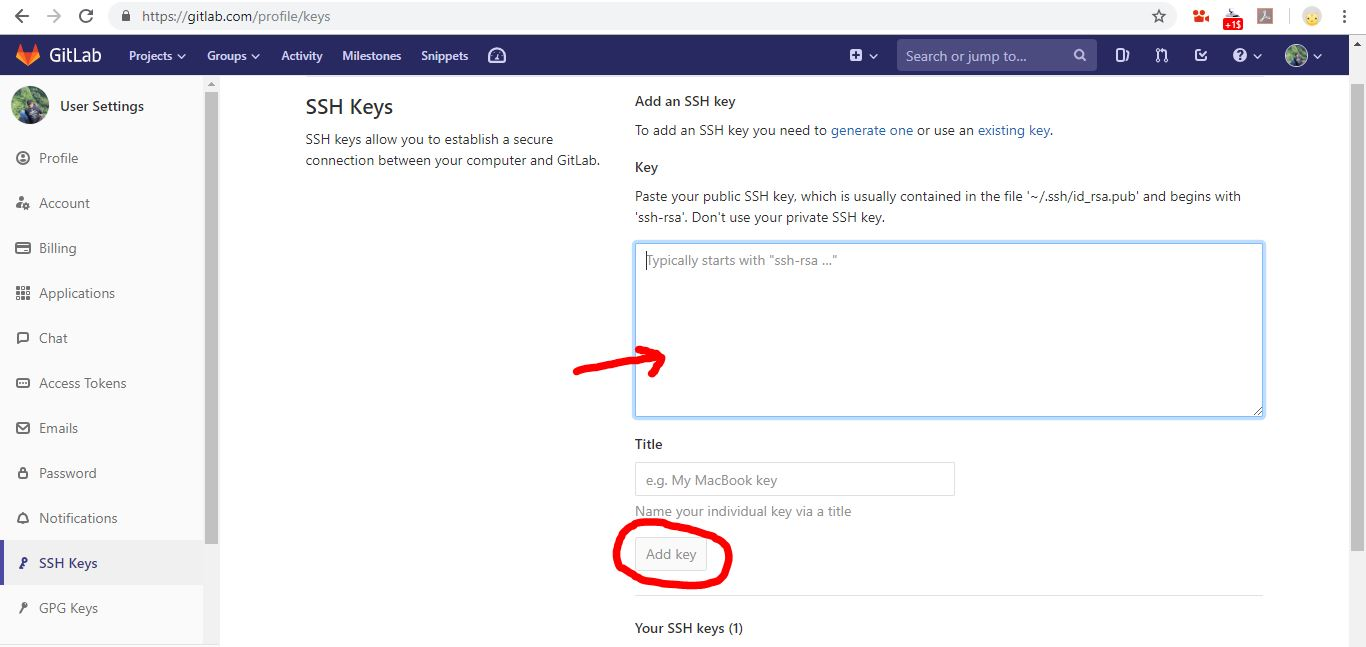
\includegraphics[width=.75\textwidth]{Figures/gitlab/SettingSSH.JPG}}
\caption{Pengisian Form SSH Key Pada Gitlab}
\label{fig:k2}
\end{figure}
\end{enumerate}